\chapter{Platform as a Service with Openshift}
\label{cha:paas}
Platform as a Service (PaaS) is a cloud service which provides an on demand platform for building, deploying and running containerized applications in the cloud. PaaS can be seen as an enhancement of CaaS, which has been discussed in the former Chapter \vref{cha:caas}. A PaaS platform does not only provide a container runtime for running containers in the cloud but also tooling for building, deploying and monitoring of containerized applications as well as security mechanisms for securing those applications. There are multiple PaaS providers on the market but the most popular PaaS providers are RedHat Openshift Online, Microsoft Azure Cloud Services, Google App Engine and AWS Elastic Beanstalk. They all bring in their own flavor of PaaS but they all provide similar features necessary by an PaaS platform \cite{OpenshiftOnline2018, MicrosoftAzueCloudServices2018, GoogleCloudAE2018, AmazonWebServicesEBT2018}. \\

PaaS providers usually provide templates for the major programming languages and application servers, and integration to other cloud services as well. External cloud services of the same vendor are usually better supported than cloud services of other vendors. This is normal, because cloud providers want the developers to use their service over the services of the competition. What all PaaS providers have in common is the consumption based pricing model, where only the consumed physical resources have to be paid for. \\ 

IPaaS can be seen as an enhancement of PaaS which is suitable for implementing an ESB which is discussed in Chapter \vref{cha:esb}. IPaaS enhances an ordinary PaaS platform by providing tooling for integrating external service effortlessly, via a low/no code platform, where services can be integrated via an UI, rather then by implementing source code. RedHat JBoss Fuse 7 is an example for an IPaaS platform which will replace JBoss Fuse 6.x in the near future \cite{Fuse72018, iPaaSP12015, iPaaSP22015}. \\

Openshift Origin is an open source PaaS platform, which has been released in April 2012 and is the upstream project for Openshift. Before Openshift 3 (Jun 2013), Openshift used its own container runtime and orchestration tooling, which since Openshift 3 have been replaced by Docker and Kubernetes, because of its popularity and general availability. Openshift is the only major PaaS platform of the formerly noted ones which can be self hosted or hosted by a local provider. The other formerly noted PaaS providers such as Microsoft Azure are only available as a cloud service hosted in the vendors data centers \cite{OpenshiftOriginGithub2018}.

\section{The need for Platform as a Service}
\label{sec:paas-need-for-paas}
As mentioned in Section \vref{sec:caas-kubernetes-worker}, there are some use cases where Kubernetes or in particular CaaS is not suitable anymore. CaaS is suitable if its used by developers, but not for persons without any deep knowledge of Docker and Kubernetes. This is where PaaS platforms come into place, which provide a web console and a template mechanism, which can be used by non-developers. Developers specify templates for the provided services which contains all technical parts of a service infrastructure and non-developers provide values for the exposed parameters which are non-technical, and the PaaS platform instantiates the template and deploys the service infrastructure automatically. \\

Enterprises can profit from PaaS platforms by defining templates for services they provide for their departments, partners or customers, who can create an instance of a provided service on demand, and destroy it if not needed anymore. PaaS platforms provide a self service console, where services can be created, managed and destroyed effortlessly without the need to understand the underlying technology. The self service console could be implemented by enterprises for their specific use cases, where the self service console interacts with PaaS platform via its exposed API. \\

PaaS platforms like Openshift usually provide an integration in a Continuous Integration / Continuous Deployment (CI/CD) workflow, which allows to automatically build and deploy new service releases in the PaaS platform automatically via web hooks. Therefore, the PaaS platforms are integrated in the whole software life cycle. This decreases the effort of the developers to interact with the cloud platform and provide additional automation.
 
\section{Openshift}
\label{sec:paas-openshift}
Openshift is a open source PaaS platform, which uses Docker and Kubernetes for the Docker Container orchestration. Openshift is designed as a client server architecture and a master slave architecture, the same way as a Kubernetes Cluster, which has been discussed in Section \vref{sec:caas-kubernetes}. An Openshift Cluster can contain multiple Kubernetes Clusters which are managed by a Openshift Master-Node, which is discussed in Section \vref{sec:paas-openshift-master}, which manages the Kubernetes Master-Nodes. Openshift provides Openshift Projects, which are discussed in Section \vref{sec:paas-openshift-project}, which place all defined resources in a Kubernetes namespace, and which are isolated form each other. The following Figure \vref{fig:paas-openshift-kubernetes-cluster-architecture} illustrates the architecture of an Openshift Cluster \cite{OpenshiftDeepDive2014, OpenshiftCoreConcepts2018}.

\newpage

\begin{figure}[htbp]
	\centering
	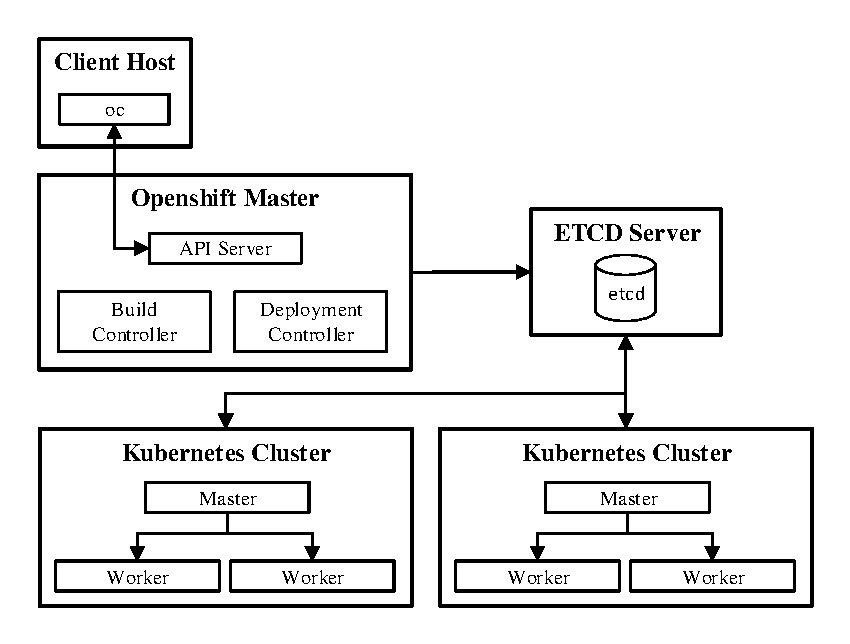
\includegraphics[scale=1]{images/openshift-kubernetes-cluster-architecture.pdf}
	\caption{Architecture of a Openshift Cluster}
	\label{fig:paas-openshift-kubernetes-cluster-architecture}
\end{figure} 

\subsection{Openshift Master}
\label{sec:paas-openshift-master}
The Openshift Maser-Node manages the Kubernetes Master-Nodes of the Kubernetes Clusters the Openshift Cluster contains. The Openshift Master exposes a REST-API via the clients can interact with the Openshift Cluster. Therefore that Openshift is placed on top of Kubernetes, the Openshift Master-Node acts similar as a Kubernetes-Master-Node, which has been discussed in Section \vref{sec:caas-kubernetes-master}. Additionally Openshift provides features Kubernetes does not, such as a role and group based security model for isolating the Kubernetes Namespaces via Openshift Projects and controllers for managing the additional Openshift Objects. The following Section \vref{sec:paas-openshift-project} discusses Openshift Projects, which are the main feature provided by Openshift.

\subsection{Openshift Project}
\label{sec:paas-openshift-project}
An Openshift Project represents a Kubernetes namespace, where all resources of an Openshift Project are located. An Openshift Project provides the isolation and security Kubernetes Namespaces do not provide. The Figure \vref{fig:paas-openshift-project-architecture} illustrates the Openshift Project-Architecture, its contained Objects and their dependency to each other. The bold marked objects within the Project representing the Openshift Objects which are provided by Openshift.

\begin{figure}[htbp]
	\centering
	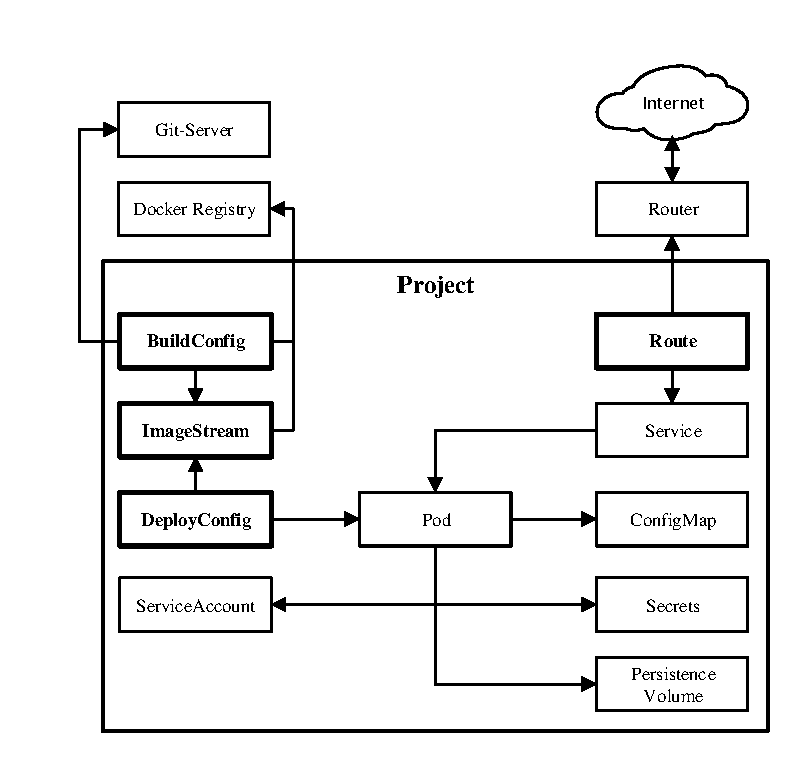
\includegraphics[scale=1]{images/openshift-project-architecture.pdf}
	\caption{Architecture of a Openshift Project}
	\label{fig:paas-openshift-project-architecture}
\end{figure} 

Openshift Objects are persistent objects in the Openshift System, and the Openshift Objects describe the state of the Openshift Cluster. This behavior has been inherited from the underlying Kubernetes System as discussed in Section \vref{sec:caas-kubernetes-objects}. The following sections briefly introduce the new Objects provided by Openshift. 

\mysubsubsection{BuildConfig}
A Build Configuration specifies the way how a Docker Image is built on the Openshift platform. The built Docker Image is pushed into the Openshift internal Docker Registry. Openshift Build Configurations support the following listed strategies:
\begin{itemize}
	\item The \emph{Source-to-Image (S2I)} strategy is the build strategy which builds a Docker Image from source code.
	\item The \emph{Docker} strategy is the build strategy which builds a Docker Image from a Dockerfile.
	\item The \emph{Custom} strategy is the build strategy which build a Docker Image with a custom implemented build mechanism.
	\item The \emph{Pipeline} strategy is the build strategy which performs a Jenkins pipeline build on a Jenkins build server.
\end{itemize}
The necessary resources for the particular build strategy are provided via a git repository, and a Build Configuration can be triggered by an external service such as Github via a web hook \cite{S2I2018}. 

\mysubsubsection{ImageStream}
An Image Stream and its Image Stream-Tags are an abstraction of the actual used Docker Image and an Image Stream uses the same naming convention as Docker Tags (E.g \mentionedtext{myproject/app:1.0}), where
\begin{itemize}
	\item \mentionedtext{myproject} represents the Image Stream namespace,
	\item \mentionedtext{app} represents the Image Stream name and
	\item \mentionedtext{1.0} represents the Image Stream-Tag.
\end{itemize}
An Image Stream-Tag references the actual Docker Image by its tag. Once the Docker Image has been imported, it will not be automatically pulled again unless the Image Stream-Tag has the name \mentionedtext{latest} which causes Openshift to always to pull the referenced Docker Image. \\

A Docker Image can be updated in a Docker Registry, which would break the consistency principle, because it wouldn't be the same Docker Image as used before the update. An Image Stream or in particular the Image stream-Tag prevents this, by referencing the actual Docker Image instance instead of only referencing the Docker Image by its tag. This approach makes the Docker Image immutable within a Openshift Project, unless the latest version is explicitly defined.  \\

\mysubsubsection{DeployConfig}
A Deployment Configuration specifies how a deployment of an Pod has to be performed. A Deployment Configuration allows to specify the Kubernetes life cycle hooks pre-hook or post-hook, which are used to configure the deployed Pod before its process has started (pre-hook) or after its process has started and is ready (post-hook). Deployment Configurations support the following listed deployment strategies:
\begin{itemize}
	\item The \emph{Rolling} strategy is the deployment strategy which waits for the new deployment to be ready before the old deployment gets removed.
	\item The \emph{Recreate} strategy is the deployment strategy which removes the old deployment when the new deployment gets started.
	\item The \emph{Custom} strategy is the deployment strategy which performs the deployment by a custom implementation.
\end{itemize}

\mysubsubsection{Route}
A Route exposes a Service with a host name to an external network (mostly the Internet), so that it can be reached by its host name from clients located outside of the Openshift Cluster. The Route is deployed on a Openshift Router, which performs the routing between the external network and the connected Service. A Route can be secured with TLS, where the certificates of the Openshift Cluster can be used or the certificate can directly be defined in the Route definition. \\